% !TEX root = smc_bandits.tex

We assess below the impact of Monte Carlo sample size $M$ in the performance of the proposed SMC-based Bayesian MAB policies
in Scenario E defined by Equation~\eqref{eq:linear_mixing_dynamics_e},
for a realization of expected rewards as depicted in Figure~\ref{fig:linear_mixing_dynamics_e_softmax}.

% Scenario E
\begin{figure}[!h]
\centering
\begin{subfigure}[b]{0.45\textwidth}
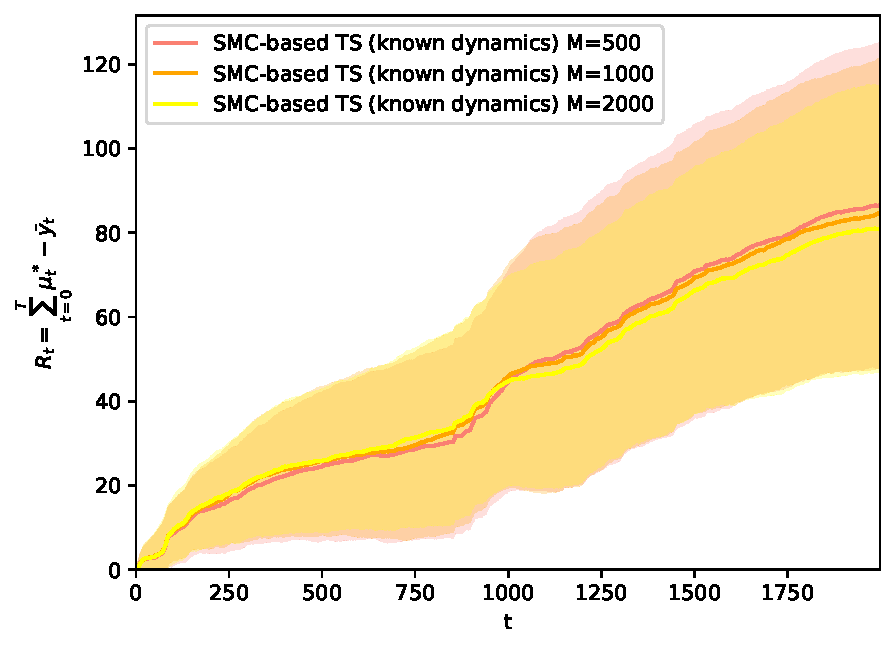
\includegraphics[width=\textwidth]{./fods_figs/dynamic/softmax/e_selectedM_cumulative_regret_dknown_ts}
\caption{Cumulative regret for SMC-based TS in scenario E: known dynamic parameters.}
\label{fig:dynamic_bandits_softmax_e_ts_dknown_M}
\end{subfigure}\qquad
\begin{subfigure}[b]{0.45\textwidth}
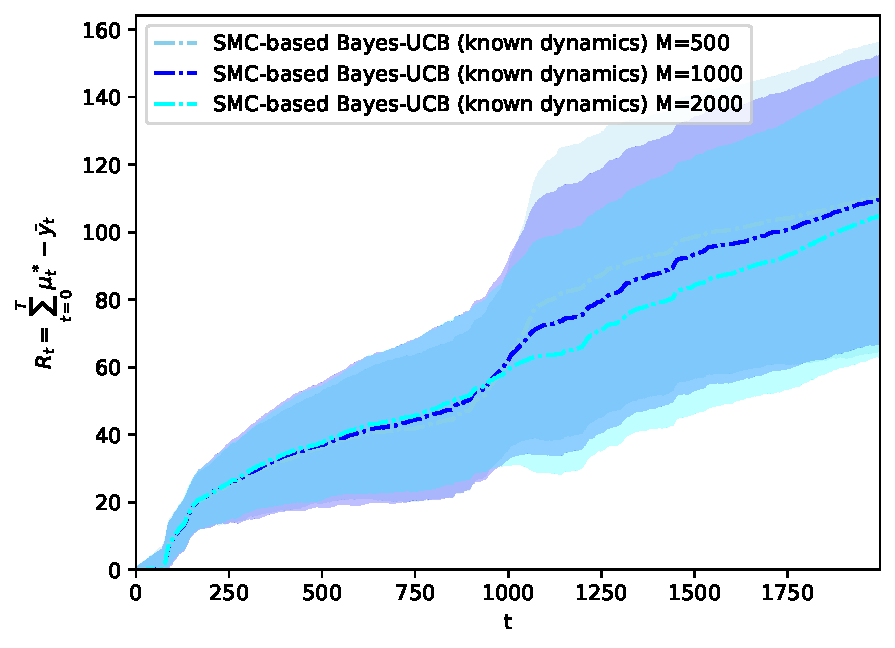
\includegraphics[width=\textwidth]{./fods_figs/dynamic/softmax/e_selectedM_cumulative_regret_dknown_bucb}
\caption{Cumulative regret for SMC-based Bayes-UCB in scenario E: known dynamic parameters.}
\label{fig:dynamic_bandits_softmax_e_bucb_dknown_M}
\end{subfigure}

\begin{subfigure}[b]{0.45\textwidth}
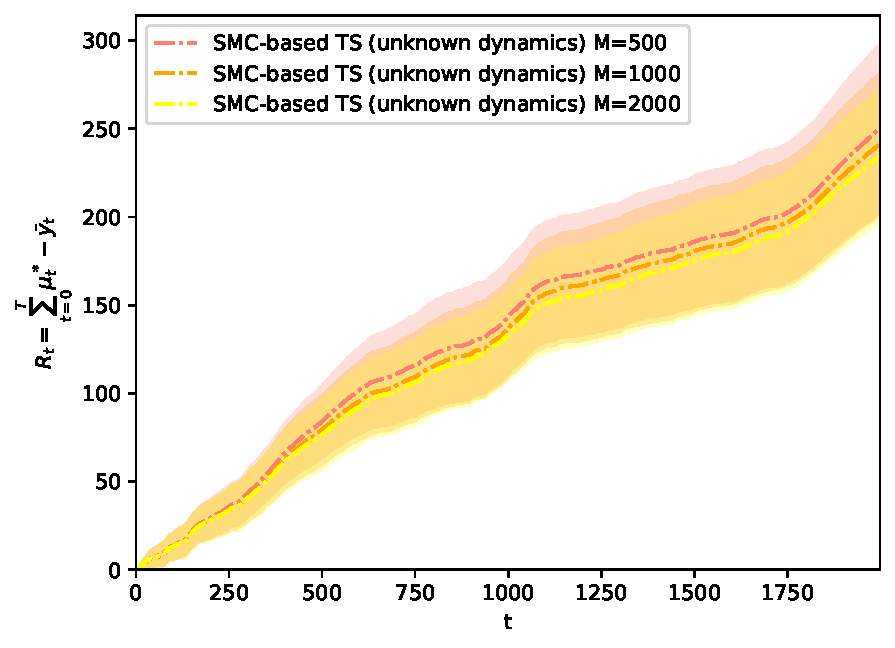
\includegraphics[width=\textwidth]{./fods_figs/dynamic/softmax/e_selectedM_cumulative_regret_dunknown_ts}
\caption{Cumulative regret for SMC-based TS in scenario E: unknown dynamic parameters $L_a,\Sigma_a,\sigma_a^2, \forall a$.}
\label{fig:dynamic_bandits_softmax_e_ts_dunknown_M}
\end{subfigure}\qquad
\begin{subfigure}[b]{0.45\textwidth}
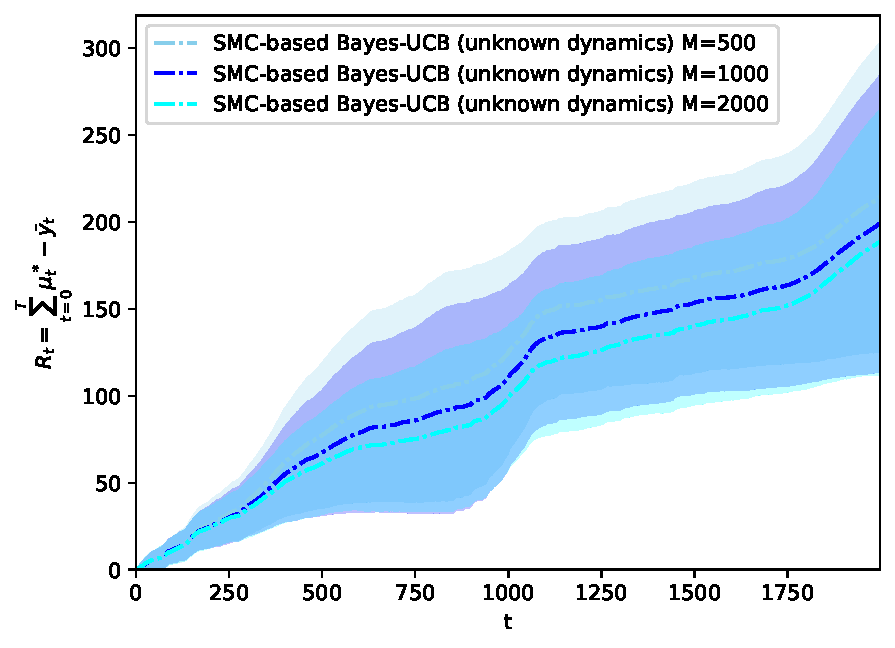
\includegraphics[width=\textwidth]{./fods_figs/dynamic/softmax/e_selectedM_cumulative_regret_dunknown_bucb}
\caption{Cumulative regret for SMC-based Bayes-UCB in scenario E: unknown dynamic parameters $L_a,\Sigma_a,\sigma_a^2, \forall a$.}
\label{fig:dynamic_bandits_softmax_e_bucb_dunknown_M}
\end{subfigure}

\caption{
Mean regret (standard deviation shown as the shaded region) in contextual, softmax bandit Scenario E
described in Equation~\eqref{eq:linear_mixing_dynamics_e}.
SMC-based policies' averaged cumulative regret is robust to different Monte Carlo sample sizes $M$,
which slightly impacts the performance variability for $M=500$.
}
\label{fig:dynamic_bandits_softmax_e_M}
\end{figure}

\clearpage
We assess below the impact of Monte Carlo sample size $M$ in the performance of the proposed SMC-based Bayesian MAB policies
in Scenario F defined by Equation~\eqref{eq:linear_mixing_dynamics_f},
for a realization of expected rewards as depicted in Figure~\ref{fig:linear_mixing_dynamics_f_softmax}.

% Scenario F
\begin{figure}[!h]
\centering
\begin{subfigure}[b]{0.45\textwidth}
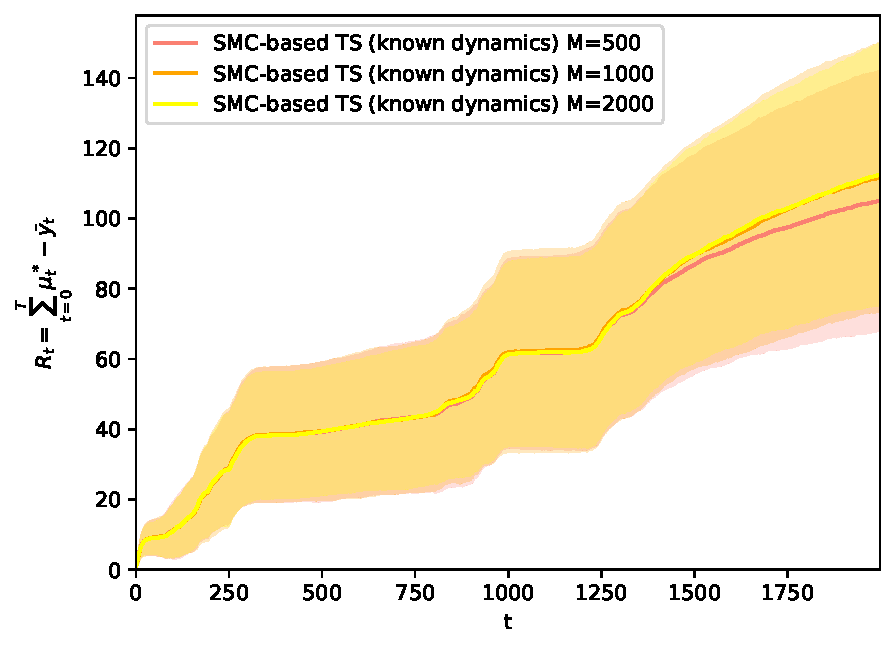
\includegraphics[width=\textwidth]{./fods_figs/dynamic/softmax/f_selectedM_cumulative_regret_dknown_ts}
\caption{Cumulative regret for SMC-based TS in scenario F: known dynamic parameters.}
\label{fig:dynamic_bandits_softmax_f_ts_dknown_M}
\end{subfigure}\qquad
\begin{subfigure}[b]{0.45\textwidth}
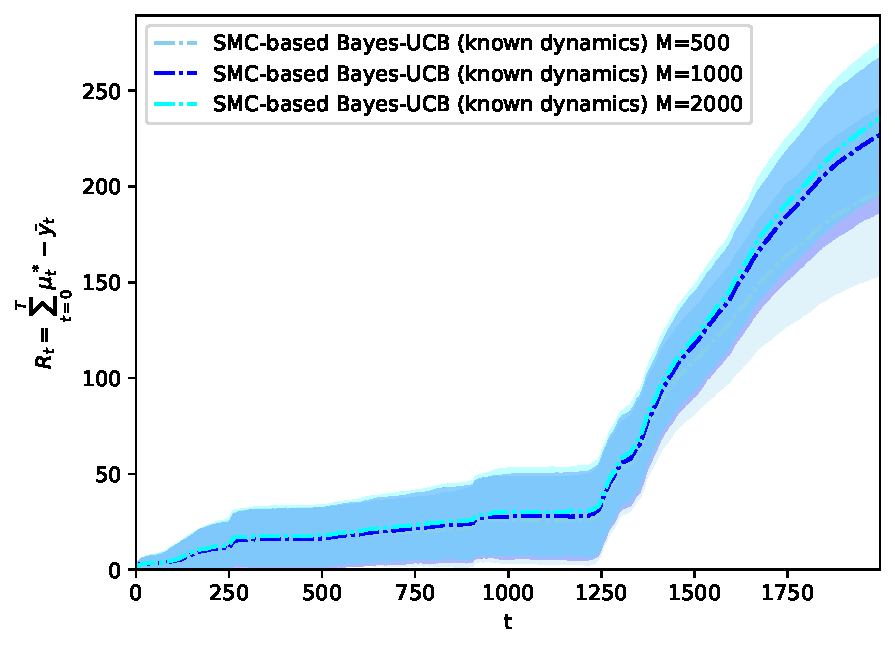
\includegraphics[width=\textwidth]{./fods_figs/dynamic/softmax/f_selectedM_cumulative_regret_dknown_bucb}
\caption{Dumulative regret for SMC-based Bayes-UCB in scenario F: known dynamic parameters.}
\label{fig:dynamic_bandits_softmax_f_bucb_dknown_M}
\end{subfigure}

\begin{subfigure}[b]{0.45\textwidth}
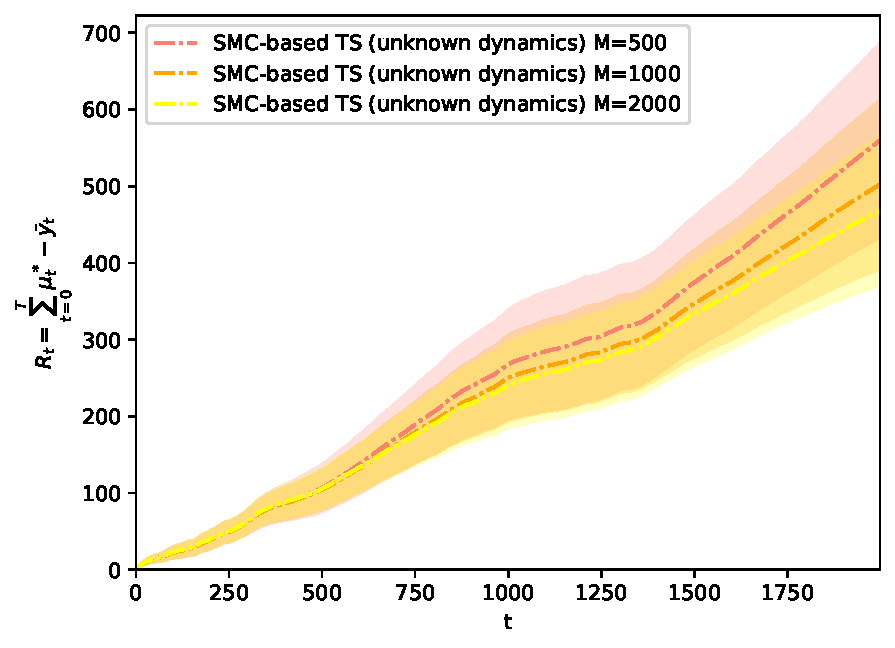
\includegraphics[width=\textwidth]{./fods_figs/dynamic/softmax/f_selectedM_cumulative_regret_dunknown_ts}
\caption{Cumulative regret for SMC-based TS in scenario F: unknown dynamic parameters $L_a,\Sigma_a,\sigma_a^2, \forall a$.}
\label{fig:dynamic_bandits_softmax_f_ts_dunknown_M}
\end{subfigure}\qquad
\begin{subfigure}[b]{0.45\textwidth}
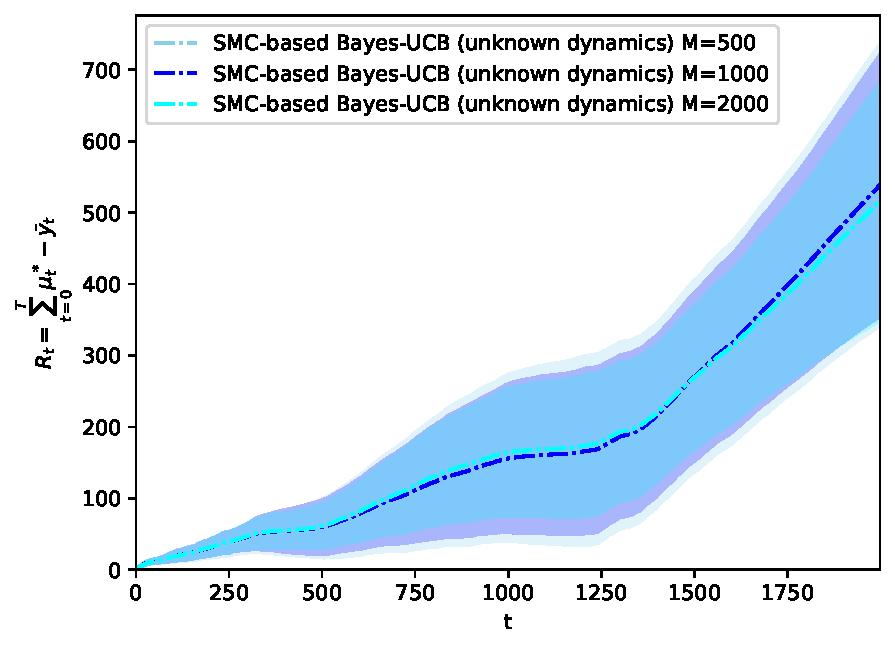
\includegraphics[width=\textwidth]{./fods_figs/dynamic/softmax/f_selectedM_cumulative_regret_dunknown_bucb}
\caption{Cumulative regret for SMC-based Bayes-UCB in scenario F: unknown dynamic parameters $L_a,\Sigma_a,\sigma_a^2, \forall a$.}
\label{fig:dynamic_bandits_softmax_f_bucb_dunknown_M}
\end{subfigure}

\caption{
Mean regret (standard deviation shown as the shaded region) in contextual, softmax bandit Scenario F
described in Equation~\eqref{eq:linear_mixing_dynamics_f}.
SMC-based policies' averaged cumulative regret is robust to different Monte Carlo sample sizes $M$,
which slightly impacts the performance variability for $M=500$.
}
\label{fig:dynamic_bandits_softmax_f_M}
\end{figure}
